% Copyright 2010 by Nicholas Bartlett

\documentclass{beamer}
\usepackage{algorithm}
\usepackage{algorithmic}
\usepackage[numbers]{natbib}

% Setup appearance:

\usetheme{Darmstadt}
%\usetheme{Copenhagen}
\usefonttheme[onlylarge]{structurebold}
\setbeamerfont*{frametitle}{size=\normalsize,series=\bfseries}
\setbeamertemplate{navigation symbols}{}

% Standard packages
\usepackage[english]{babel}
%\usepackage[latin1]{inputenc}
%\usepackage{times}
%\usepackage[T1]{fontenc}
%\usepackage{nnfootnote}
\usepackage{amsfonts}
\usepackage{amsmath}
%\newcommand{\argmax}{\operatornamewithlimits{argmax}}
\def\newblock{\hskip .11em plus .33em minus .07em}
% Setup TikZ

%\usepackage{tikz}
%\usetikzlibrary{arrows}
%\tikzstyle{block}=[draw opacity=0.7,line width=1.4cm]

\bibliographystyle{plainnat}

% Author, Title, etc.

\title[Forgetting Counts: A Constant Memory Approach to Online Prediction of a Discrete Sequence] 
{
	Forgetting Counts: A Constant Memory Approach to Online Prediction of a Discrete Sequence
}

\author[Bartlett]
{
  Nicholas~Bartlett %\inst{1}
}

\institute[Columbia University]
{
  %\inst{1}%
  Columbia University
}

\date[Apr 17, 2010]
{Apr 17, 2010}

%\def\blfootnote{\xdef\@thefnmark{}\@footnotetext}

% The main document
% !TEX root = talk.tex

\newcommand{\comment}[1]{}
%\newcommand{\comment}[1]{{\marginpar{\tiny {#1} }}}
\def\todo#1{TODO(#1)}

\def\bigO{{\mathcal O}}
\def\balpha{\mbox{\boldmath $\alpha$}}
\def\bbeta{\mbox{\boldmath $\beta$}}
\def\beeta{\mbox{\boldmath $\eta$}}
\def\blambda{\mbox{\boldmath $\lambda$}}
\def\bmu{\mbox{\boldmath $\mu$}}
\def\bphi{\mbox{\boldmath $\phi$}}
\def\bpsi{\mbox{\boldmath $\psi$}}
\def\bsigma{\mbox{\boldmath $\sigma$}}
\def\btau{\mbox{\boldmath $\tau$}}
\def\btheta{\mbox{\boldmath $\theta$}}
\def\dbphi{\dot{\mbox{\boldmath $\phi$}}}
\def\dbtau{\dot{\mbox{\boldmath $\tau$}}}
\def\dbtheta{\dot{\mbox{\boldmath $\theta$}}}

%\newcommand{\nofootnotemark}{\let\@makefnmark\relax}
\newcommand{\bX}{\mathbf{X}}
\newcommand{\bY}{\mathbf{Y}}
\newcommand{\bW}{\mathbf{W}}
\newcommand{\bZ}{\mathbf{Z}}
\newcommand{\bH}{\mathbf{H}}
\newcommand{\bQ}{\mathbf{Q}}
\newcommand{\bA}{\mathbf{A}}
\newcommand{\bI}{\mathbf{I}}
\newcommand{\by}{\mathbf{y}}
\newcommand{\bz}{\mathbf{z}}
\newcommand{\bx}{\mathbf{x}}

\newcommand{\ith}{i^\mathrm{th}}
\def\A{{\bf A}}
\def\B{{\bf B}}
\def\C{{\bf C}}
\def\D{{\bf D}}
\def\F{{\bf F}}
\def\L{{\bf L}}
\def\M{{\bf M}}
\def\W{{\bf W}}
\def\I{{\bf I}}
\def\J{{\bf J}}
\def\R{{\bf R}}
\def\U{{\bf U}}
\def\V{{\bf V}}
\def\b{{\bf b}}
\def\c{{\bf c}}
\def\d{{\bf d}}
\def\r{{\bf r}}
\def\s{{\bf s}}
\def\t{{\bf t}}
\def\u{{\bf u}}
\def\v{{\bf v}}
\def\f{{\bf f}}
\def\x{{\bf x}}
\def\y{{\bf y}}
\def\w{{\bf w}}
\def\vo{{\bf o}}
\def\p{{\bf p}}
\def\O{{\bf 0}}
%\def\a{{\bf a}}


\def\vbpsi{\vec{\mbox{\boldmath $\psi$}}} 
\def\vpsi{\vec{\psi}} 
\def\vbphi{\vec{\mbox{\boldmath $\phi$}}} 
\def\vphi{\vec{\phi}} 
\def\vbtau{\vec{\mbox{\boldmath $\tau$}}} 
\def\vbtheta{\vec{\mbox{\boldmath $\theta$}}} 
\def\vD{\vec{D}}
\def\vf{\vec{\bf f}}
\def\vF{\vec{\bf F}}
\def\vI{\vec{\bf I}}
\def\vR{\vec{\bf R}}
\def\vv{\vec{v}}
\def\vV{\vec{\bf V}}

\def\pon{p_{\mathrm{on}}}
\def\poff{p_{\mathrm{off}}}

\def\tr{^{\text{T}}}

%%% Vector notation for sections 3 and 4
%%% Vector notation for sections 3 and 4
\def\mvec{\vec{m}}
\def\fvec{\vec{f}}
\def\appfvec{\vec{f}_k}
\def\avec{\vec{a}}
\def\bvec{\vec{b}}
\def\evec{\vec{e}}
\def\uvec{\vec{u}}
\def\xvec{\vec{x}}
\def\wvec{\vec{w}}
\def\gradvec{\vec{\nabla}}

\def\aM{\mbox{\bf a}_M}
\def\aS{\mbox{\bf a}_S}
\def\aO{\mbox{\bf a}_O}
\def\aL{\mbox{\bf a}_L}
\def\aP{\mbox{\bf a}_P}
\def\ai{\mbox{\bf a}_i}
\def\aj{\mbox{\bf a}_j}
\def\an{\mbox{\bf a}_n}
\def\a1{\mbox{\bf a}_1}
\def\a2{\mbox{\bf a}_2}
\def\a3{\mbox{\bf a}_3}
\def\a4{\mbox{\bf a}_4}

%\def\x{\mbox{\bf x\/}}
%\def\X{\mbox{\bf X}}
%\def\A{\mbox{\bf A}}
%\def\P{\mbox{\bf P}}
%\def\C{\mbox{\bf C}}
%\def\c{\mbox{\bf c}}
%\def\b{\mbox{\bf b}}
%\def\o{\mbox{\bf o}}
%\def\h{\mbox{\bf h}}
%\def\f{\mbox{\bf f}}
%\def\x{\mbox{\bf x}}
%\def\sx{\mbox{\scriptsize\bf x}}
%\def\z{\mbox{\bf z}}
%\def\l{\mbox{\bf l}}
%\def\m{\mbox{\bf m}}
%\def\bi{\mbox{\bf i}}
%\def\u{\mbox{\bf u}}
%\def\v{\mbox{\bf v}}
\def\a{\mbox{\bf a}}
%\def\p{\mbox{\bf p}}
%\def\r{\mbox{\bf r}}
%\def\d{\mbox{\bf d}}
%\def\Q{\mbox{\bf Q}}
%\def\s{\mbox{\bf s}}
%\def\st{\mbox{\scriptsize\bf t}}
%\def\ss{\mbox{\scriptsize\bf s}}
%\def\t{\mbox{\bf t}}
%\def\cR{{\cal R}}
%\def\calD{{\cal D}}
%\def\calS{{\cal S}}
%\def\g{\mbox{\bf g}}
%\def\e{\mbox{\bf e}}
%\def\flow{\{\mbox{\bf u}\}}
%\def\appearChange{iconic change}

\def\sigmae{\sigma}
\def\sigmam{\sigma}

\newcommand{\eg}{e.\thinspace{}g.,\@\xspace}
\newcommand{\egn}{e.\thinspace{}g.\@\xspace}
\newcommand{\cf}{cf.\@\xspace}
\newcommand{\ie}{i.\thinspace{}e.,\@\xspace}
\newcommand{\ien}{i.\thinspace{}e.\@\xspace}
\newcommand{\iid}{i.\thinspace{}i.\thinspace{}d.\@\xspace}


%\newcommand{\comment}[1]{}
\newcommand{\ponedec}{\mathcal{P}^\downarrow_1}
\newcommand{\pone}{\mathcal{P}_1}
\newcommand{\rank}[1]{\mathrm{RANK}\left[#1\right]}
\newcommand{\E}[1]{\mathrm{E}\left[#1\right]}
%\newcommand{\PY}{\mathcal{PY}}
%\newcommand{\DP}{\mathcal{DP}}
%\newcommand{\iid}{iid.}
\newcommand{\drawiid}{\stackrel{\text{iid}}{\sim}}
\newcommand{\vect}[1]{\mathbf{#1}}
\newcommand{\indicator}[1]{\text{I}\left[ #1 \right]}
\newcommand{\pdcoag}{PD(d_1,0)-\text{COAG}}
%\newcommand{\todo}{\textbf{*TODO*}}
\newcommand{\igram}{\text{$\infty$-gram}}
\newcommand{\Prob}{\text{P}}

\def\mm{sequence memoizer }
\def\MM{SM }

\def\pibf{{\boldsymbol{\pi}}}
\def\kapbf{\boldsymbol{\kappa}}
\def\taubf{\boldsymbol{\tau}}
\def\thebf{\boldsymbol{\theta}}
\def\rhobf{\boldsymbol{\rho}}
\def\phibf{\boldsymbol{\phi}}
\def\pbf{\mathbf{p}}
\def\qbf{\mathbf{q}}
\def\sbf{\mathbf{s}}
\def\tbf{\mathbf{t}}
\def\ybf{\mathbf{y}}
\def\ubf{\mathbf{u}}
\def\Ave{\mathbb{E}}

\def\wbf{\mathbf{w}}
\def\xbf{\mathbf{x}}
\def\rbf{\mathbf{r}}
\def\tbf{\mathbf{t}}
\def\kbf{\mathbf{k}}
\def\Xbf{\mathbf{X}}
\def\0bf{\mathbf{0}}
\def\Ibf{\mathbf{I}}
\def\phibf{\mathbf{\phi}}
\def\Phibf{\mathbf{\Phi}}
\def\disteq{{\stackrel{D}{=}}}
\def\EE{{\mathbb{E}}}
\def\GG{\mathcal{G}}
\def\G{G}
\def\U{U}

\def\phiv{\varphi}
\def\phivbf{\boldsymbol{\varphi}}

\def\Ocal{\mathcal{O}}
\DeclareMathOperator*{\Var}{Var}

\DeclareMathOperator*{\Bet}{Beta}
\DeclareMathOperator{\coag}{COAG}
\DeclareMathOperator{\frag}{FRAG}
\DeclareMathOperator*{\rnk}{RANK}
\DeclareMathOperator*{\gem}{GEM}
\DeclareMathOperator*{\pd}{PD}
\DeclareMathOperator*{\py}{PY}
\DeclareMathOperator*{\DP}{DP}
\DeclareMathOperator*{\PY}{PY}
\DeclareMathOperator*{\gd}{GDir}
\DeclareMathOperator*{\Dir}{Dir}
\DeclareMathOperator*{\CRP}{CRP}
\DeclareMathOperator*{\argmax}{argmax}



%%% Local Variables: 
%%% mode: latex
%%% TeX-master: "paper"
%%% End: 
% !TEX root = talk.tex
%
%\newcommand{\comment}[1]{}
%%\newcommand{\comment}[1]{{\marginpar{\tiny {#1} }}}
%
%\def\bigO{{\mathcal O}}
%\def\balpha{\mbox{\boldmath $\alpha$}}
%\def\bbeta{\mbox{\boldmath $\beta$}}
%\def\beeta{\mbox{\boldmath $\eta$}}
%\def\blambda{\mbox{\boldmath $\lambda$}}
%\def\bmu{\mbox{\boldmath $\mu$}}
%\def\bphi{\mbox{\boldmath $\phi$}}
%\def\bpsi{\mbox{\boldmath $\psi$}}
%\def\bsigma{\mbox{\boldmath $\sigma$}}
%\def\btau{\mbox{\boldmath $\tau$}}
%\def\btheta{\mbox{\boldmath $\theta$}}
%\def\dbphi{\dot{\mbox{\boldmath $\phi$}}}
%\def\dbtau{\dot{\mbox{\boldmath $\tau$}}}
%\def\dbtheta{\dot{\mbox{\boldmath $\theta$}}}
%
%%\newcommand{\nofootnotemark}{\let\@makefnmark\relax}
%\newcommand{\bX}{\mathbf{X}}
%\newcommand{\bY}{\mathbf{Y}}
%\newcommand{\bW}{\mathbf{W}}
%\newcommand{\bZ}{\mathbf{Z}}
%\newcommand{\bH}{\mathbf{H}}
%\newcommand{\bQ}{\mathbf{Q}}
%\newcommand{\bA}{\mathbf{A}}
%\newcommand{\bI}{\mathbf{I}}
%\newcommand{\by}{\mathbf{y}}
%\newcommand{\bz}{\mathbf{z}}
%\newcommand{\bx}{\mathbf{x}}
%
%\newcommand{\ith}{i^\mathrm{th}}
%\def\A{{\bf A}}
%\def\B{{\bf B}}
%\def\C{{\bf C}}
%\def\D{{\bf D}}
%\def\F{{\bf F}}
%\def\L{{\bf L}}
%\def\M{{\bf M}}
%\def\W{{\bf W}}
%\def\I{{\bf I}}
%\def\J{{\bf J}}
%\def\R{{\bf R}}
%\def\U{{\bf U}}
%\def\V{{\bf V}}
%\def\b{{\bf b}}
%\def\c{{\bf c}}
%\def\d{{\bf d}}
%\def\r{{\bf r}}
%\def\s{{\bf s}}
%\def\t{{\bf t}}
%\def\u{{\bf u}}
%\def\v{{\bf v}}
%\def\f{{\bf f}}
%\def\x{{\bf x}}
%\def\y{{\bf y}}
%\def\w{{\bf w}}
%\def\vo{{\bf o}}
%\def\p{{\bf p}}
%\def\O{{\bf 0}}
%%\def\a{{\bf a}}
%
%
%\def\vbpsi{\vec{\mbox{\boldmath $\psi$}}} 
%\def\vpsi{\vec{\psi}} 
%\def\vbphi{\vec{\mbox{\boldmath $\phi$}}} 
%\def\vphi{\vec{\phi}} 
%\def\vbtau{\vec{\mbox{\boldmath $\tau$}}} 
%\def\vbtheta{\vec{\mbox{\boldmath $\theta$}}} 
%\def\vD{\vec{D}}
%\def\vf{\vec{\bf f}}
%\def\vF{\vec{\bf F}}
%\def\vI{\vec{\bf I}}
%\def\vR{\vec{\bf R}}
%\def\vv{\vec{v}}
%\def\vV{\vec{\bf V}}
%
%\def\pon{p_{\mathrm{on}}}
%\def\poff{p_{\mathrm{off}}}
%
%\def\tr{^{\text{T}}}
%
%%%% Vector notation for sections 3 and 4
%%%% Vector notation for sections 3 and 4
%\def\mvec{\vec{m}}
%\def\fvec{\vec{f}}
%\def\appfvec{\vec{f}_k}
%\def\avec{\vec{a}}
%\def\bvec{\vec{b}}
%\def\evec{\vec{e}}
%\def\uvec{\vec{u}}
%\def\xvec{\vec{x}}
%\def\wvec{\vec{w}}
%\def\gradvec{\vec{\nabla}}
%
%\def\aM{\mbox{\bf a}_M}
%\def\aS{\mbox{\bf a}_S}
%\def\aO{\mbox{\bf a}_O}
%\def\aL{\mbox{\bf a}_L}
%\def\aP{\mbox{\bf a}_P}
%\def\ai{\mbox{\bf a}_i}
%\def\aj{\mbox{\bf a}_j}
%\def\an{\mbox{\bf a}_n}
%\def\a1{\mbox{\bf a}_1}
%\def\a2{\mbox{\bf a}_2}
%\def\a3{\mbox{\bf a}_3}
%\def\a4{\mbox{\bf a}_4}
%
%%\def\x{\mbox{\bf x\/}}
%%\def\X{\mbox{\bf X}}
%%\def\A{\mbox{\bf A}}
%%\def\P{\mbox{\bf P}}
%%\def\C{\mbox{\bf C}}
%%\def\c{\mbox{\bf c}}
%%\def\b{\mbox{\bf b}}
%%\def\o{\mbox{\bf o}}
%%\def\h{\mbox{\bf h}}
%%\def\f{\mbox{\bf f}}
%%\def\x{\mbox{\bf x}}
%%\def\sx{\mbox{\scriptsize\bf x}}
%%\def\z{\mbox{\bf z}}
%%\def\l{\mbox{\bf l}}
%%\def\m{\mbox{\bf m}}
%%\def\bi{\mbox{\bf i}}
%%\def\u{\mbox{\bf u}}
%%\def\v{\mbox{\bf v}}
%\def\a{\mbox{\bf a}}
%%\def\p{\mbox{\bf p}}
%%\def\r{\mbox{\bf r}}
%%\def\d{\mbox{\bf d}}
%%\def\Q{\mbox{\bf Q}}
%%\def\s{\mbox{\bf s}}
%%\def\st{\mbox{\scriptsize\bf t}}
%%\def\ss{\mbox{\scriptsize\bf s}}
%%\def\t{\mbox{\bf t}}
%%\def\cR{{\cal R}}
%%\def\calD{{\cal D}}
%%\def\calS{{\cal S}}
%%\def\g{\mbox{\bf g}}
%%\def\e{\mbox{\bf e}}
%%\def\flow{\{\mbox{\bf u}\}}
%%\def\appearChange{iconic change}
%
%\def\sigmae{\sigma}
%\def\sigmam{\sigma}
%
%\newcommand{\eg}{e.\thinspace{}g.,\@\xspace}
%\newcommand{\egn}{e.\thinspace{}g.\@\xspace}
%\newcommand{\cf}{cf.\@\xspace}
%\newcommand{\ie}{i.\thinspace{}e.,\@\xspace}
%\newcommand{\ien}{i.\thinspace{}e.\@\xspace}
%\newcommand{\iid}{i.\thinspace{}i.\thinspace{}d.\@\xspace}
%
%
%%\newcommand{\comment}[1]{}
%\newcommand{\ponedec}{\mathcal{P}^\downarrow_1}
%\newcommand{\pone}{\mathcal{P}_1}
%\newcommand{\rank}[1]{\mathrm{RANK}\left[#1\right]}
%%\newcommand{\E}[1]{\mathrm{E}\left[#1\right]}
%%\newcommand{\PY}{\mathcal{PY}}
%%\newcommand{\DP}{\mathcal{DP}}
%%\newcommand{\iid}{iid.}
%\newcommand{\drawiid}{\stackrel{\text{iid}}{\sim}}
%\newcommand{\vect}[1]{\mathbf{#1}}
%\newcommand{\indicator}[1]{\text{I}\left[ #1 \right]}
%\newcommand{\pdcoag}{PD(d_1,0)-\text{COAG}}
%%\newcommand{\todo}{\textbf{*TODO*}}
%\newcommand{\igram}{\text{$\infty$-gram}}
%\newcommand{\Prob}{\text{P}}
%
%\def\mm{sequence memoizer }
%\def\MM{SM }
%
%\def\pibf{{\boldsymbol{\pi}}}
%\def\kapbf{\boldsymbol{\kappa}}
%\def\taubf{\boldsymbol{\tau}}
%\def\thebf{\boldsymbol{\theta}}
%\def\rhobf{\boldsymbol{\rho}}
%\def\phibf{\boldsymbol{\phi}}
%\def\pbf{\mathbf{p}}
%\def\qbf{\mathbf{q}}
%\def\sbf{\mathbf{s}}
%\def\tbf{\mathbf{t}}
%\def\ybf{\mathbf{y}}
%\def\ubf{\mathbf{u}}
%\def\Ave{\mathbb{E}}
%
%\def\wbf{\mathbf{w}}
%\def\xbf{\mathbf{x}}
%\def\rbf{\mathbf{r}}
%\def\tbf{\mathbf{t}}
%\def\kbf{\mathbf{k}}
%\def\Xbf{\mathbf{X}}
%\def\0bf{\mathbf{0}}
%\def\Ibf{\mathbf{I}}
%\def\phibf{\mathbf{\phi}}
%\def\Phibf{\mathbf{\Phi}}
%\def\disteq{{\stackrel{D}{=}}}
%\def\GG{\mathcal{G}}
%\def\G{G}
%\def\U{U}
%
%\def\phiv{\varphi}
%\def\phivbf{\boldsymbol{\varphi}}
%
%\def\Ocal{\mathcal{O}}
%\DeclareMathOperator*{\Var}{Var}
%
%\DeclareMathOperator*{\Bet}{Beta}
%\DeclareMathOperator{\coag}{COAG}
%\DeclareMathOperator{\frag}{FRAG}
%\DeclareMathOperator*{\rnk}{RANK}
%\DeclareMathOperator*{\gem}{GEM}
%\DeclareMathOperator*{\pd}{PD}
%\DeclareMathOperator*{\py}{PY}
%\DeclareMathOperator*{\DP}{DP}
%\DeclareMathOperator*{\PY}{PY}
%\DeclareMathOperator*{\gd}{GDir}
%\DeclareMathOperator*{\Dir}{Dir}
%\DeclareMathOperator*{\CRP}{CRP}
%\DeclareMathOperator*{\argmax}{argmax}
%
\def\GG{\mathcal{G}}
\def\data{\mathbf{x}}
%\def\EE{\mathbb{E}}
\def\disc{d}
%\newcommand{\delete}[1]{} %\textcolor{red}{#1}
%\newcommand{\rewrite}[1]{#1}%{\textcolor{blue}{#1}} %
%\newcommand{\lambdabf}{\boldsymbol{\lambda}}
%\newcommand{\vbf}{\mathbf{v}}
%\newcommand{\Psmooth}{\Prob_\text{smooth}}
%%\newcommand{\parent}{\pi}
%\newcommand{\suffix}{\sigma}
%\newcommand{\UHPYP}{SM}
%\newcommand{\PLUMP}{PLUMP}
%\newcommand{\Oh}{\mathcal{O}}
%\newcommand{\tree}{\mathcal{T}}
\newcommand{\cct}{\hat{\mathcal{T}}}
\newcommand{\cctx}{\cct(\data)}
\newcommand{\Gu}{G_{\ubf}}
%\newcommand{\GuSet}{\{G_{\ubf}\}_{\ubf \in \Sigma^*}}
%\newcommand{\E}{\mathrm{E}}
%\newcommand{\UpdatePath}{\text{\textsc{UpdatePath}}}
%\newcommand{\Path}{\ensuremath{(\ubf_0,\ldots,\ubf_P)}}
%\newcommand{\PathProbability}{\text{\textsc{PathProbability}}}
%\newcommand{\TT}{\mathcal{T}}
%\newcommand{\ral}[1]{\stackrel{\mathtt{#1}}{\rightarrow}}
\def\parent{{\sigma(\mathbf{u})}}
%
%%\def\newblock{\hskip .11em plus .33em minus .07em}
%
%
%% \newcommand{\cusk}{c_{\ubf s k}}
%% \newcommand{\cus}{c_{\ubf s \cdot}}
%% \newcommand{\cu}{c_{\ubf \cdot \cdot}}
%% \newcommand{\tus}{t_{\ubf s}}
%% \newcommand{\tu}{t_{\ubf \cdot}}
%\newcommand{\cusk}{c_{\ubf s k}}
%\newcommand{\cus}{c_{\ubf s}}
%\newcommand{\cu}{c_{\ubf \cdot}}
%\newcommand{\tus}{t_{\ubf s}}
%\newcommand{\tu}{t_{\ubf \cdot}}
%\newcommand{\cset}{\{\cusk\}_{s\in \Sigma,k \in \{1,\ldots,t_{\ubf s}\}}}
%\newcommand{\tset}{\{\tus\}_{s\in \Sigma}}
%\newcommand{\bydef}{\equiv}
%\newcommand{\state}{\mathcal{S}_{\xbf}}
%\newcommand{\statei}{\mathcal{S}_{\xbf_{1:i}}}
%%\newcommand{\emptystring}{\varepsilon}
%\newcommand{\gcount}{\hat{c}}
%\newcommand{\escape}{\mathtt{esc}}
%\def\prob{G}
%
%
%\newcommand{\todo}[1]{\begin{center}\textbf{TODO: } #1 \end{center}}
%\newcommand{\figref}[1]{\figurename~\ref{#1}}
%\newcommand{\predictive}{\Prob(x_i|\xbf_{1:i-1})}
%\newcommand{\ywcomment}[1]{\textbf{#1}}
%\newcommand{\jgcomment}[1]{ { \textcolor{red}{#1} } }
%
%\newcommand{\secref}[1]{Section \ref{#1}}
%
\def\context{\mathbf{u}}

%%% Local Variables: 
%%% mode: latex
%%% TeX-master: "paper"
%%% End: 


\begin{document}

\begin{frame}
	\titlepage
\end{frame}

\section{Introduction}
\subsection{Motivation}

\begin{frame}{Data: Stream of Discrete Observations}
	\begin{block}{Byte Stream}
		\[
		\begin{array}{l}
			01001001 , 01101110 , 00100000 , 01110100,\\
			01101000 , 01110010 , 01100101 , 01100101,\\
			00100000 , 01100100 , 01100001 , 01111001,\\
			01110010 , 01100001 , 01110011 , 01101000\ldots
		\end{array}
		\]
	\end{block}
	
	\begin{block}{Word Stream}
		\[
		\begin{array}{l}
			{\rm the, rabbit, hole, went, straight, on, like, a, tunnel, for, some}\\
			{\rm way, and, then, dipped, suddenly, down, so, suddenly, that}\\
			{\rm  alice, had, not, a, moment, to, think, about, stopping, herself}\\
			{\rm  before, she, found, herself, falling, down, a, very, deep, well}
		\end{array}
		\]
	\end{block}
\end{frame}

\begin{frame}{Task}
	\begin{block}{Prediction}
		Given a sequence of discrete observations $X_1, \ldots, X_n$, predict the next observation $X_{n+1}$.
	\end{block}
	
	\begin{block}{Requirements}
		\begin{itemize}
			\item{Linear time estimation in the length of the sequence}
			\item{Constant time prediction}
			\item{Constant space memory complexity}
		\end{itemize}
	\end{block}
	
	\begin{block}{Challenges}
		\begin{itemize}
			\item{Sparse Data}
			\item{Categorical Data}
			\item{Complex Generative Mechanism}
		\end{itemize}
	\end{block}
\end{frame}

\begin{frame}{Example Applications}
	\begin{itemize}
		\item{Natural Language}
		\begin{itemize}
			\item Words, i.e.~the united \_
			\item Characters, i.e.~un\_
			\item Parts of speech, i.e.~NNV\_
		\end{itemize}

		\vspace{.75cm}		
		
		\item{Compression}
		\begin{itemize}
			\item  Bits i.e.~0101000011110001\_
			\item  Bytes i.e.~6A7B4ED22100D\_
		\end{itemize}
		
		\item \ldots
	\end{itemize}
\end{frame}

\subsection{Approach}

\begin{frame}{Tools}
	\begin{itemize}
		\item Model : hierarchical Bayesian nonparametrics \cite{Teh2006b}
		\begin{itemize}
			\item Bayesian regularization
			\item Immediate, closed-form posterior sampling
			\item Flexible distributional form
			\item Hierarchically composable
		\end{itemize}
		
		\item Incremental inference : \cite{Doucet2001,Liu2001,MacEachern1999}
		\begin{itemize}
			\item  Sequential Monte Carlo,  \cite{Wood2007,Wood2008,Wood2008b,Gasthaus2010}
		\end{itemize}

		\item Constant memory complexity.
		\begin{itemize}
			\item Coagulation / fragmentation operators \cite{Pitman1999,Ho2006}
			\item Forgetting, \citet{Bartlett2010}
		\end{itemize}
	\end{itemize}
\end{frame}	

\section{Pitman-Yor Process (PYP)}
\subsection{PYP Prior}

\begin{frame}{Pitman-Yor Process Prior}
	The Pitman-Yor Process (PYP) is a stochastic process defined such that sample paths are distribution functions over some sample space $\mathcal{X}$ with probability one \cite{Pitman1997} .  PYP priors are used in Bayesian models to replace a less flexible parametric prior.
	
	\vspace{.65cm}

	\begin{block}{Model}
		\[
		\begin{array}{rcll}
			\G | d, c, \G_0 &\sim& \PY(d,c,\G_0) &\\
			X_i | \G &\sim& \G \hspace{1cm} &\forall i
		\end{array}
		\]
	\end{block}
	
	The PYP can also be hierarchically composed and will be denoted HPYP \cite{teh2006a}
\end{frame}

\begin{frame}{Drawing $\{ X_i \}_{i =1}^n$}
	\begin{block}{Process}
		\begin{itemize}
			\item Draw a partition of the first $n$ natural numbers from the two parameter Ewen's Sampling Distribution ($\ES_n(d,c)$) \cite{Ewens1995}.
			\vspace{.5cm}
			\item Assign a value $\psi_t \sim \G_0$ to part $t$ of the partition.
			\vspace{.5cm}
			\item Set $X_i = \psi_t$ if $i$ is in the $t^{\rm th}$ part of the partition.
		\end{itemize}
	\end{block}
\end{frame}

\subsection{Ewen's Sampling Distribution}

\begin{frame}{$\ES_n(d,c)$}
	\begin{block}{Drawing from $\ES_n(d,c)$ (Urn Representation)}
		\begin{itemize}
			\item Assign the integer $1$ to part $1$ of the partition.
			\item {For $i = 2, \ldots, n$, assign integer $i$ to a part drawn from the following distribution: \\
				\vspace{-.65cm}
				\begin{eqnarray*}
					p({\rm part~}t \leq k_{i-1}  | {\rm previous~assignments}) &=& \frac{n_t - d}{i-1 + c}\\
					p({\rm  part~} k_{i-1} + 1 | {\rm previous~ assignments}) &=& \frac{k_{i-1}d + c}{i-1 + c}\\
				\end{eqnarray*}
				\noindent where $k_{i-1}$ is the number of partitions to which the first $i-1$ integers have been assigned.
			}
			\item{Resulting partition follows $\ES_n(d,c)$  \cite{Pitman1995}}.
		\end{itemize}
	\end{block}
\end{frame}

\section{Dependent PYP and HPYP}
\subsection{Construction}

\begin{frame}{Consistency of $\ES$ Under Deletion}
	\begin{block}{Property}
		If an integer is removed at random from a partition following $\ES_n(d,c)$ the resulting partition of $n-1$ integers follows $\ES_{n-1}(d,c)$  \cite{Pitman1995}.
	\end{block}
	
	\begin{block}{Application}
		This consistency property can be exploited in a generative procedure defined using the urn representation to draw samples from a sequence of dependent distributions $\{ \G^t \}_{t = 1}^T$ such that 
		\[
		\begin{array}{rcll}
			\G_t | d,c,\G_0 &\sim& \PY(d,c,\G_0)& t = 1, \ldots, T\\
			X_i^t | \G^t &\sim& \G^t& i = 1, \ldots, N_t, t = 1, \ldots, T
		\end{array}
		\]
	\end{block}
\end{frame}

\begin{frame}[t] {Dependent HPYP Depiction}
	\begin{figure}[t]
		\begin{center}
			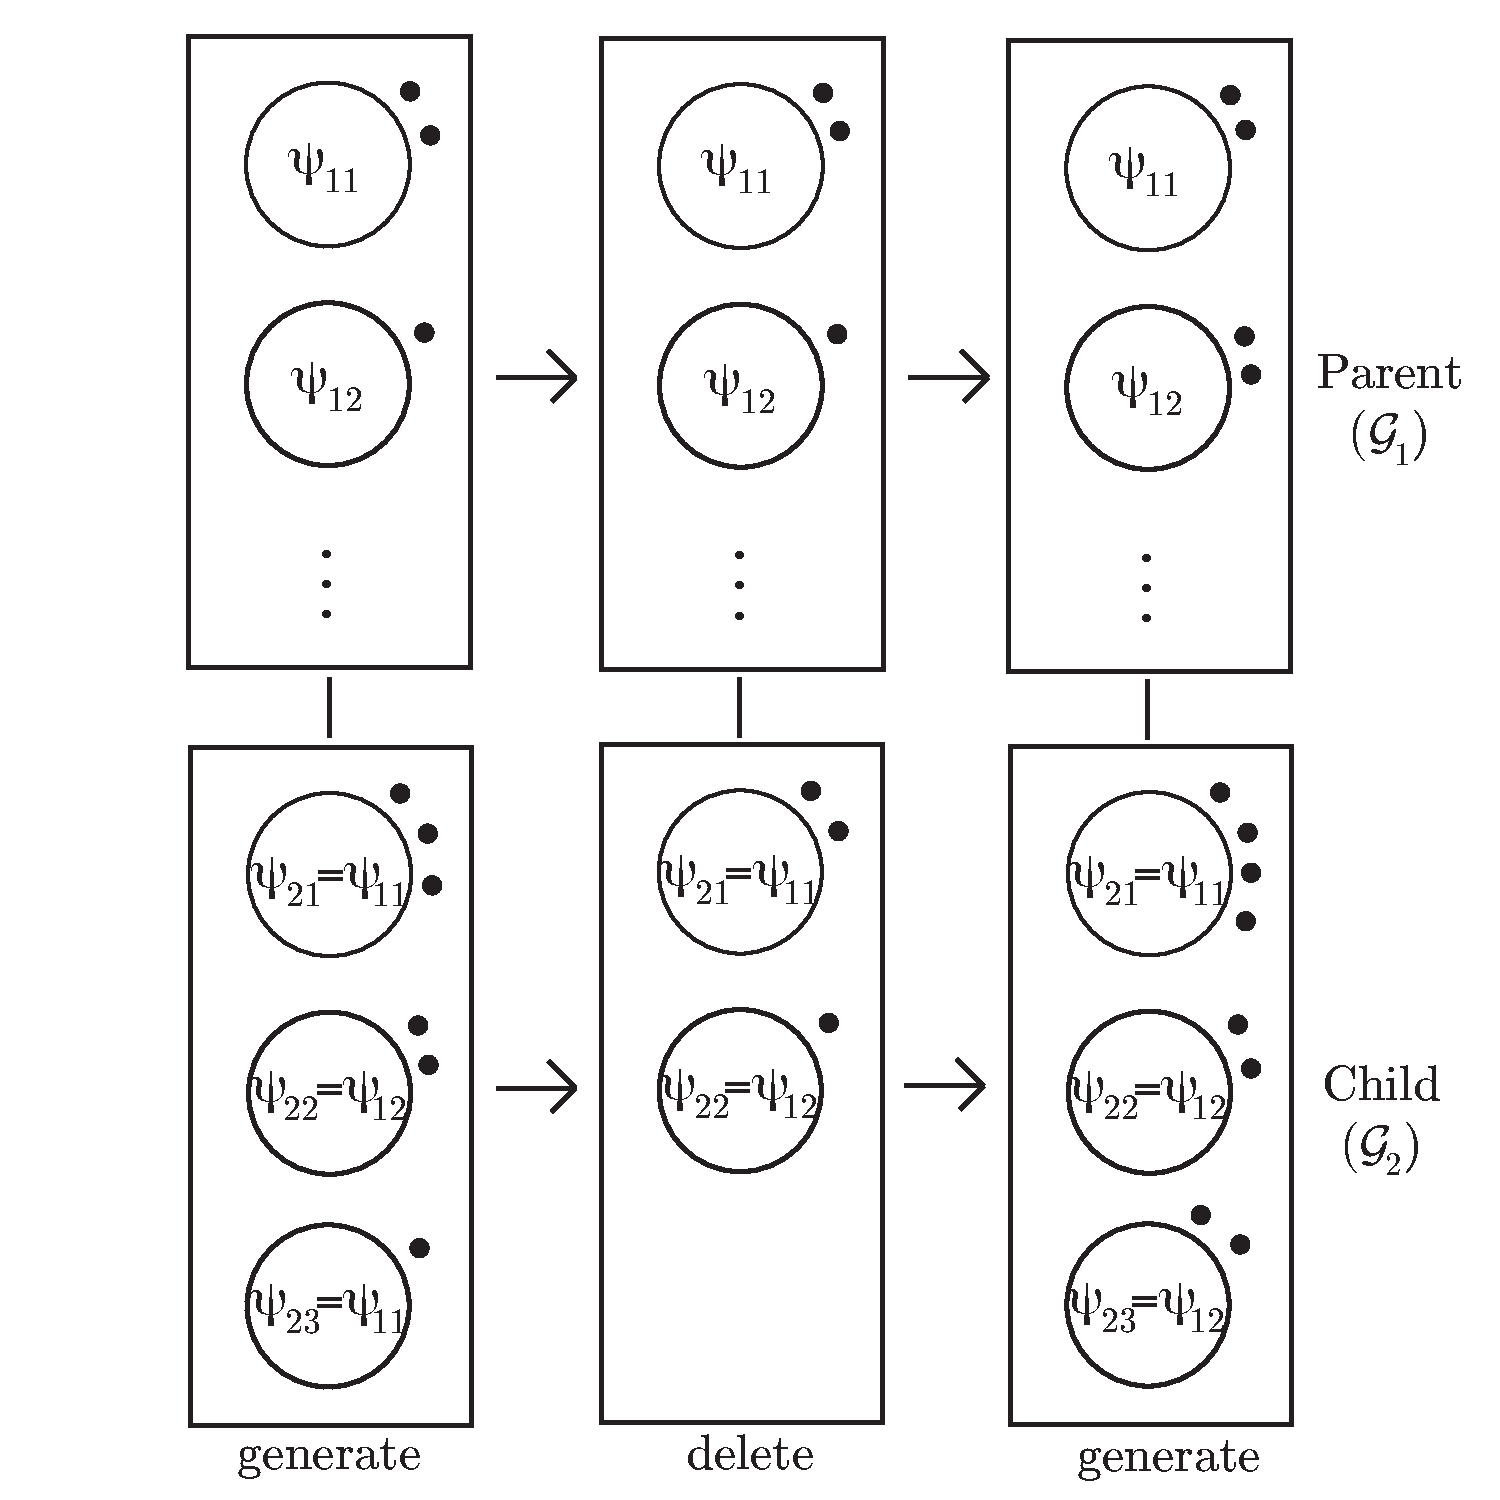
\includegraphics[width=9cm, height = 7cm]{../../papers/2010_icml/bounded_memory_compression/figure2.pdf}
		\end{center}
	\end{figure}
\end{frame}

\subsection{Sequence Memoizer}

\begin{frame}{Sequence Memoizer Model, \cite{Wood2009} }
	\begin{eqnarray*}
		\Sigma &=& \{0,1\}\\
		\U_{\Sigma } &=& [.5, .5] \\
		\\
		\G_{[]} | \U_{\Sigma}, d_0 &\sim& \PY(d_0, 0, \U_{\Sigma }) \\
		\G_{\bf{u}} | \G_{\sigma(\bf{u})}, d_{|\bf{u}|} &\sim& \PY(d_{|\bf{u}|}, 0, \G_{\sigma(\bf{u})}) \hspace{.35cm} \forall {\bf u} \in \Sigma^+\\
		x_n | x_{n-1},  \ldots, x_1 = \bf{u} &\sim& \G_{\bf{u}}
		\end{eqnarray*}

		Here $\sigma(x_1x_2x_3\ldots x_n) = x_2x_3\ldots x_n$ is the suffix operator.
\end{frame}

\begin{frame}[t] {A Way to Tie Together ``Related'' Conditional Distributions}
	\begin{figure}[htbp]
		\begin{center}
			\vspace{2cm}
			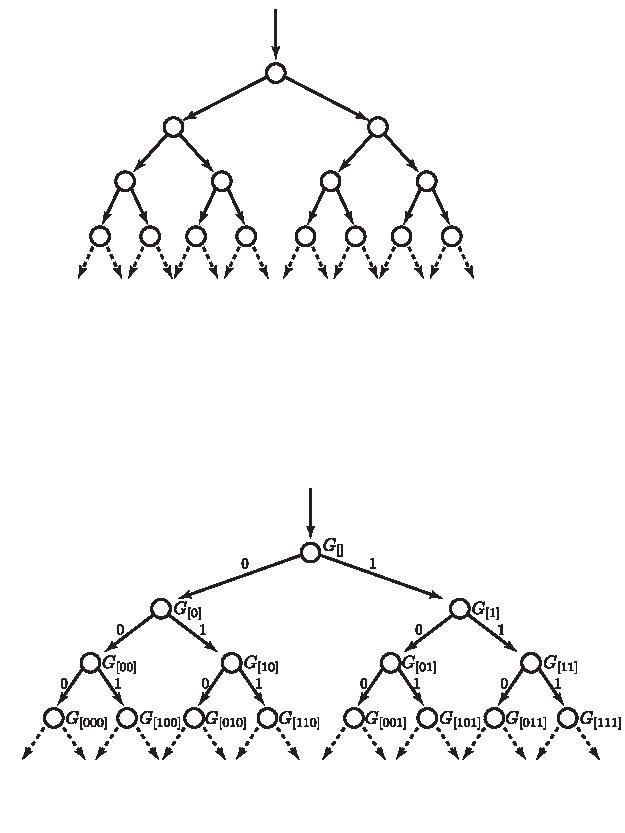
\includegraphics[trim = 2cm 2cm 2cm 10cm, width=8cm]{base.pdf}
		\end{center}
	\end{figure}
\end{frame}


\begin{frame}[t]{Computational Problems}
	\begin{itemize}
		\item Number of nodes in graphical model is $\mathcal{O}(2^n)$
		\begin{itemize}
			\item Solution : marginalize (ignore) conditional distributions not found in sequence
		\end{itemize}
		
		\item Number of conditional distributions in graphical model still grows $\mathcal{O}(n^2)$
		\begin{itemize}
			\item Solution, \cite{Wood2009} : marginalize out non-branching nodes \cite{Pitman1999, Ho2006}
			\item Use suffix tree algorithms to identify  $\mathcal{O}(n)$ remaining nodes.
		\end{itemize}
		
		\item Number of conditional distributions grows as $\mathcal{O}(n)$ but suffix tree algorithms require full sequence
		\begin{itemize}
			\item Solution, \cite{Gasthaus2010} : note (worst-case) $\mathcal{O}(n^2)$ inference time and show that incremental construction algorithm suffices
		\end{itemize}
		
		\item Number of nodes grows as $\mathcal{O}(n)$	
	\end{itemize}
\end{frame}


\subsection{Constrained Memory}

\begin{frame}{Dependent HPYP as Constrained Memory}
	``The number of instantiated nodes can be limited using the deletion scheme developed for dependent HPYP�s. Memory savings can be achieved by deleting all the elements in a leaf node since empty leaf nodes do not need to be represented" \citet{Bartlett2010}.
\end{frame}

\begin{frame}[t]{Constant Space Sequence Memoizer}
	\begin{figure}[t]
		\begin{center}
			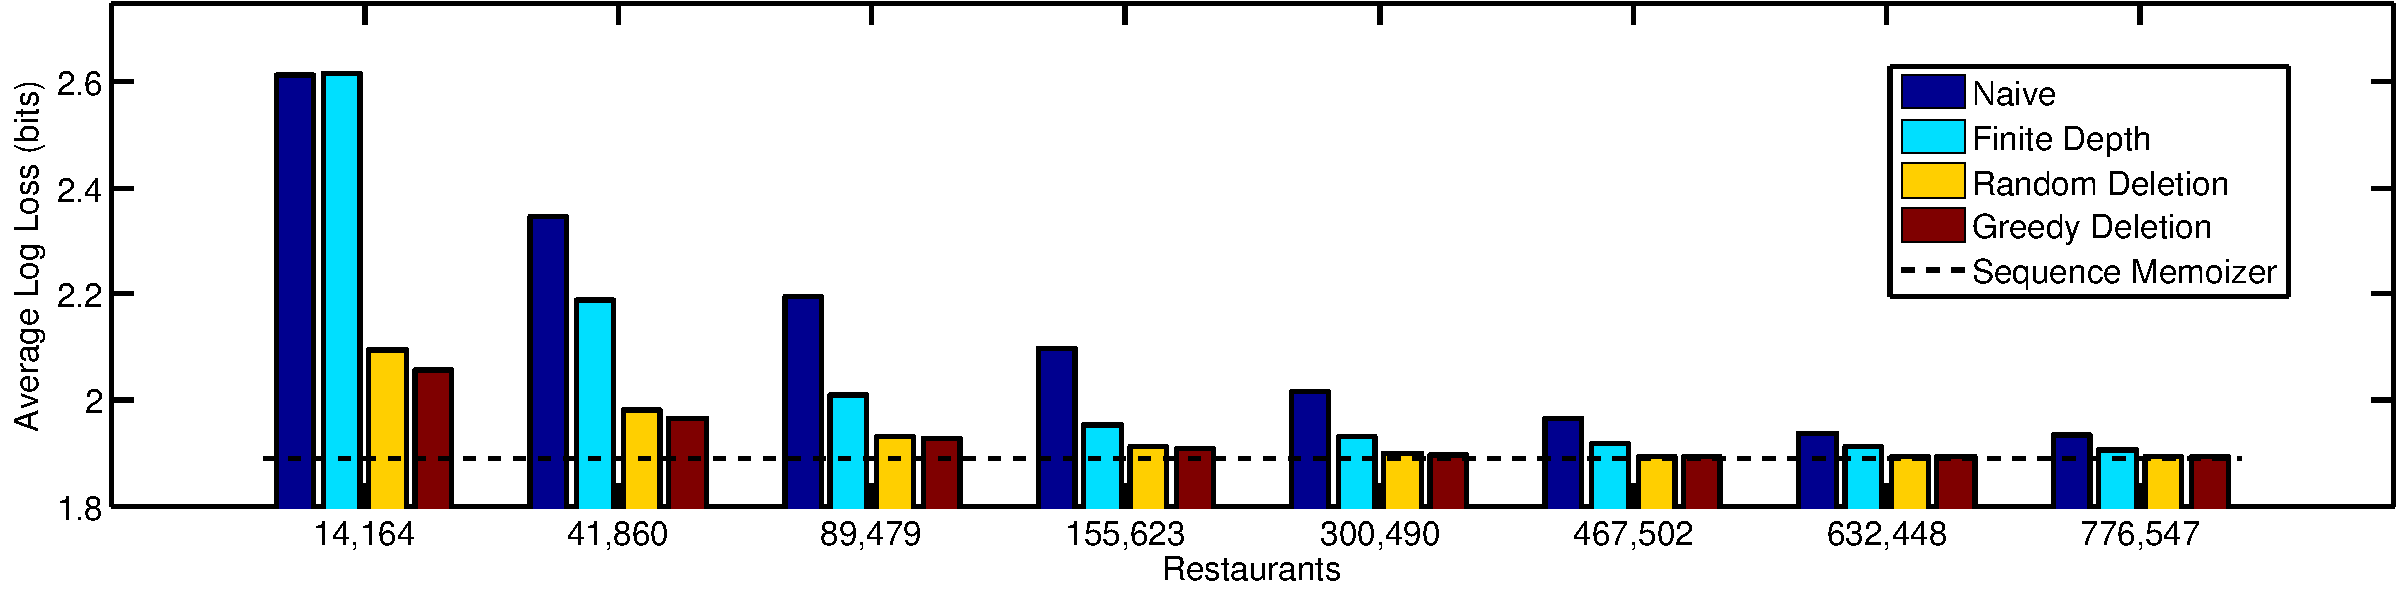
\includegraphics[width=10cm]{../../papers/2010_icml/bounded_memory_compression/results_calgary_corpus.pdf}
		\end{center}
	\end{figure}
	
	\begin{itemize}
		\item Calgary corpus
		\item Different forgetting schemes
		\item $256$ character alphabet
	\end{itemize}
\end{frame}

\begin{frame}{Thanks}
	Collaborators
	\begin{itemize}
		\item Frank Wood, Columbia University
		\item David Pfau, Columbia University
	\end{itemize}
\end{frame}

\begin{frame}[t,allowframebreaks]{Bibliograpy}
	\bibliography{../../papers/uber}
\end{frame}

\section{Appendix}

\begin{frame}[t]{Example Prefix Tree: $patat$}
	\begin{center}
		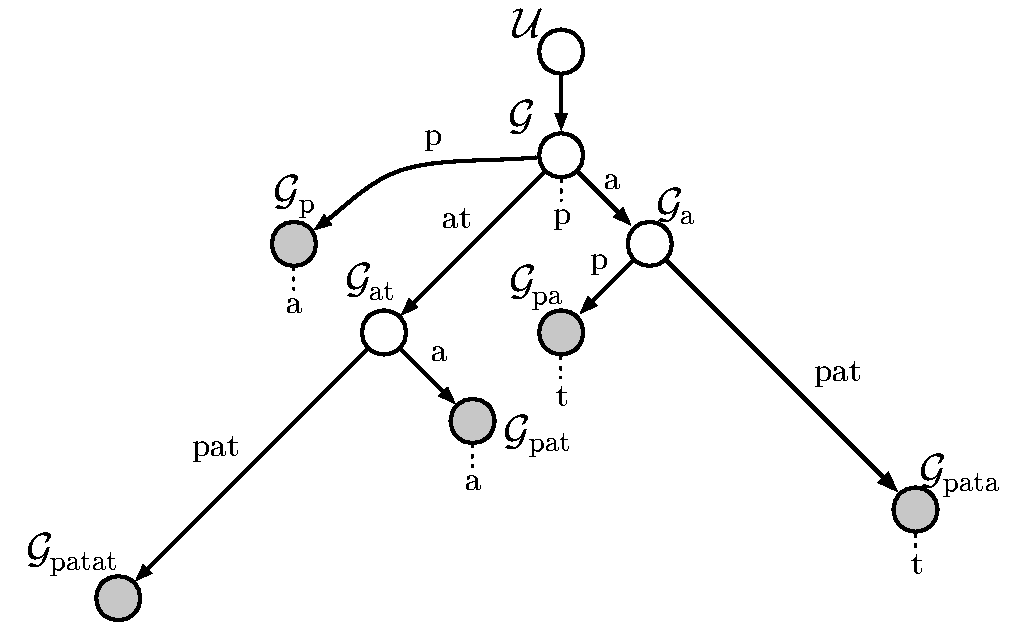
\includegraphics[width = 10cm]{../../papers/2010_icml/bounded_memory_compression/prefix_tree.pdf}
	\end{center}
\end{frame}

\begin{frame}{Example Deletion}
	``consider what would happen if we deleted all the elements in the node labeled $\G_{pa}$. Let $\G^t_{pa} = \G_{pa}$.  Implicit in this deletion is the assumption that the distribution over symbols following the context $pa$ in the sequence prior to the deletion step, $\G_{pa}^t$  is, conditioned on  $\G_a$, independent of the distribution $\G_{pa}^{t+1}$ after the deletion at time $t$" \citet{Bartlett2010}.
\end{frame}

\end{document}


